\documentclass{fisatproject}
\title{Hologram with Haptic Feedback}
\team{Leo Varghese(FIT16CS071) \\ Mohit Rajan E(FIT16CS078)\\ Riya Alexander(FIT16CS097)}
\author{Leo Varghese}
\regno{FIT16CS071}
\begin{document}
\maketitle
\makecert
\font\secfont =  cmr12 at 15pt
\newpage
\pagenumbering{roman}
\setcounter{page}{1}
\newgeometry{top=4cm,bottom=0.1cm}
\thispagestyle{plain}
\renewcommand\abstractname{ABSTRACT}
\begin{abstract}
\vspace{5cm}
This paper is intended to analyze and discuss the developments made so far in the field of holography and holographic projection, it discusses the doability and the eventuality in the field of touchable holograms, which works in gear with hand gestures. In this paper, first some elementary matters about what a hologram is and a concise description of how they are devised is discussed. Then how hologram interact with our hand gestures and provide haptic feedback is discussed. In this paper the focus is on the feasibility or doability study of some methods and the analysis and consequences of these methods. Challenges in the whole process will be confronted and then some discussion about future scopes of this technology and where this technology can lead us is done.
\end{abstract}



\newpage
\renewcommand\abstractname{Contribution by Author}
\thispagestyle{plain}
\begin{abstract}
\vspace{5cm}
I focused mainly on rendering holographic objects and researched on retargeting the object position in space. I reviewed Yiwei Zhao et al. [1] and Dan Gotsch et al. [2].
I also helped to schedule workplan for this project and to calculate the budget of the whole project.

\vspace{1cm}
\begin{flushright}
Leo Varghese
\end{flushright}
\end{abstract}

\newpage
\renewcommand\abstractname{ACKNOWLEDGMENT}
\thispagestyle{plain}
\begin{abstract}
\vspace{5cm}

If words are considered as symbols of approval and tokens of acknowledgement,then let the words play the heralding role of expressing our gratitude.First and foremost we Thank God almighty for the Grace he showered for the successful completion of our project.
\newline

We are extremely thankful to the Chairman,\textbf{Mr.Paul Mundadan}, who provided us with all the vital facilities required for the successful completion of our project.
We also thank out Principal, \textbf{Dr. George Issac} for the amenities he provided.We would like to express our sincere gratitude to Prof Dr.Prasad JC(H.O.D) who always guided us and rendered his maximum support in all phases of our project.
We are expressing our sincere gratitude to \textbf{Ms.Reshmi R} ,\textbf{ Mr.Jestin Joy} and \textbf{ Ms.Soumya S Raj},assistant professors of Department of Computer Science and Engineering for their constant support in every phase and for the source of strength in completing this work.As the project coordinators they have provided necessary assistance throughout the project. 
We would like to express our gratitude to the project in charge 
\textbf{Mr.Anuranj Pullanatt} for his constant support and encouragement and for rendering help in all phases of our project with patience and enthusiasm.
\newline
We would like to express our  sincere gratitude to all the faculties of Computer Science Department,FISAT.We would like to express special thanks to our Lab instructors for providing us with all the lab facilities and for helping us throughout to make it a success.
We also sincerely thank our parents and friends for giving us moral support and encouragement in all possible ways.
\vspace{1cm}
\begin{flushright}
Leo Varghese
\end{flushright}
\end{abstract}
\newpage

\restoregeometry
\tableofcontents
\newpage

\cleardoublepage
\addcontentsline{toc}{chapter}{\listfigurename}
\listoffigures
\newpage

\cleardoublepage
\addcontentsline{toc}{chapter}{\listtablename}
\listoftables
\newpage



\chapter{Introduction}
\pagenumbering{arabic}
\setcounter{page}{1}
\renewcommand{\baselinestretch}{1.50}
\section{Overview}
\par Haptic holography is a combination of computational modeling and spatial display.It enables a person to see, feel, and interact with free standing holographic pictures of material surfaces that is three-dimensional in nature. In this project, holographic displays are merged with a force-feedback device to render images with programmatically, real-world  material properties and behavior.

\par A method to produce haptic area in the air using spatial modulation of ultrasound is initiated. Method to create airborne ultrasonic tactile stimulation is based on vibrotactile radiation pressure and sensor feedback systems. The initiated approach produces a spatially standing haptic image that enables user to touch 3D images  depending on vibrotactile feedback.


\section{Problem Statement}

\par In the current education system students are taught to learn formulas and how to use them but not to reason or understand the logic behind them, causing then to forget it in a short period.It is a typical longitudinal learning approach. Our brain system is not just longitudinal in learning process, but much more complex. Current education system evolved on the basis of visual and auditory senses and their application leads to memorizing the content of learning rather than creating a holistic perception.
% which can be based on the enormous untapped abilities of the human brain.
It is observed that the current education system  uses mainly audio methods to teach students.
In India around 10\% of students suffer from some form of learning disability[1]. Research also point to the fact that visual working memory is better in students with learning disability rather than auditory working memory[2].
It can be inferred that a modern method of learning should be developed in order to increase the efficiency of learning process.

\par To address this issue  we propose a system which uses a hologram display with haptic feedback by the interaction of using hand gestures. This project will focus on developing a system as described above to introduce a new approach to learn basic geometry.
\newpage
\section{Objective}

To create a system which also includes somesthetic senses to learning. To achieve this a hologram display with haptic feedback is proposed. The proposed system can be used to project objects in mid-air which can be interacted by using the hand gestures to view new objects, change or modify its properties like size, view etc.
\subsection{Application}
\begin{itemize}
    \item  Education : Difficult concepts which require visual representation can be studied with less difficulty. 
    \item  Entertainment : Holographic displays with tactile feedback can be placed in entertainment events.
    \item  Simulations : Can be used for CAD Simulations.
\end{itemize}
\chapter{Literature Review}
\section{ 
  \normalsize A Functional Optimization Based Approach for Continuous 3D Retargeted Touch of Arbitrary, Complex Boundaries in Haptic Virtual Reality
}
\par Yiwei Zhao et al. [1] ,
Actuated physical props can provide haptic feedback. It leads to a sense of realism in virtual reality. However, the differences between the physical and virtual surfaces can diminish user experience. Haptic retargeting can overcome this limitation by utilizing visio-haptic effects. Investigations made earlier in haptic retargeting have focused on methods for point based position retargeting and techniques for remapping 2D shapes or simple 3D shape changes. This approach extends haptic retargeting to complex, arbitrary shapes, it provides a continuous mapping across all points on a boundary. This new approach also allows multi-finger interaction.  Functional optimization to find the ideal spatial warping function with different goals: a maximum mapping smoothness, a minimum difference between the real and virtual world, or the combination of the latter.  Preliminary user study of different optimization goals and to elaborate potential applications through a set of demonstrations is reported.
\section{\normalsize TeleHuman2: A Cylindrical Light Field Teleconferencing \\ System }
\par Dan Gotsch et al. [2],  For telepresence to support multiparty conversations, it is important to convey motion parallax and stereoscopy without head-worn apparatus. TeleHuman2 is a “hologrammatic” telepresence system. It conveys full body 3D video of interlocutors using a human-sized cylindrical light field display. For rendering, the system uses an array of projectors mounted above the heads of participants in a ring around a retroreflective cylinder. Unique angular renditions are calculated from streaming depth video captured at the remote location. Projected images are retro-reflected into the eyes of local participants, at 1.3o intervals providing angular renditions simultaneously for left and right eyes of all onlookers, which conveys motion parallax and stereoscopy without head-worn apparatus or head tracking. Our technical evaluation of the angular accuracy of the system demonstrates that the error in judging the angle of a remote arrow object represented in TeleHuman2 is within 1 degree, and not significantly different from similar judgments of a collocated arrow object.
\section{\normalsize 360-degree Transparent Holographic Screen Display}
\par Tomoharu Nakamura et al. [3], A technique for creating a sense of reality to 2D images. A holographic screen with higher transparency compared to one based on conventional technology was successfully produced. With the combination of a 360- degree transparent holographic screen display and sensing technology using multiple high-speed cameras, the observer gets the feeling that an object is “actually there”. Fusion of the background and the image increases the feeling of “floating” in the image by using a holographic screen, and the multiple high- speed cameras can make the motion parallax image according to the position of the observer in real time. Therefore, the image seems to be at the center of the cylinder.
\section{\normalsize Bringing Video Game Characters into the Real World on \\ a Holographic Light Field Display}
\par Jorge Arroyo-Palacios et al. [4],   The design and technical choices of a proof of concept migrating video game character that can move from a game environment to a holographic environment rendered on a novel holographic light field display.  These two environments with interactions that are consistent to each other, using a game controller for interaction in the game environment and voice, gesture and face tracking in the holographic environment. Finally,  a study to assess the level of social presence, consistent migration and coherent experience in our proposed system.
\section{\normalsize Ultraino: An Open Phased-Array System for Narrowband \\ Airborne Ultrasound Transmission}
\par In [6] the author has created a passed array using 40Khz ultrasonic sensors. They have demonstrated multiple example application for the same.
The haptic feedback was achieved with a semi-spherical array, which was build using transducers and 3d printed base. This design provides focal point at 2cm from the base.
An animation with 100 periods with the array on and 100 periods with  the  array  off is defined . This generated a focal point at 200Hz. This frequency is known to be more sensitive to mechanoreceptors in our skins. The focal point can be created at different positions to electronically  change  where  the  tactile  sensation  is  applied.
\chapter{Design}
\subsection{ 
  \normalsize  A Functional Optimization Based Approach for Continuous 3D Retargeted Touch of Arbitrary, Complex Boundaries in Haptic Virtual Reality
}
A new technique for haptic retargeting of complex arbitrary 3D sahpes is proposed.
By functional optimization,smoothness can be maximized,position mismatch can be minimized and both are together done.
This technique is useful when the mismatch between two boundary conditions are under just noticeable threshold.
Along with pseudo-haptic techniques,retargeting or redirecting,the process of warping is also important.
Linear mapping,position realation based 2D mapping,energy optimization mapping and mismatch and ergonomic mapping is udes to generate space warping map.
This technique is more complex compared to haptic retargeting.
This techniques allow multi-finger interaction.
Passive haptic uses already existing objects for providing haptic sensations.
Pseudo-haptic feedback is a new technique which is used in this paper.
In this,simulated haptic sensation is there which is different from real haptic feedback.
When a passive isometric input device is used along with visual feedback,a pseudo-stiffness of passive objects is produced. 
\subsection{ 
  \normalsize TeleHuman2: A Cylindrical Light Field Teleconferencing \\ System
}



TeleHuman2 is a hologrammatic telepresence system.
It provides 3D video human-sized using cylindrical light field display.
for rendering,many projectors are mounted above heads of the participants in a ring around a retroreflective cylinder.
Motion parallax is used to provide the shift of visual perspective from a interlocuter to another.
Stereoscopy is a technique that provides binocular images.
This is very important to check whether the angular depth information is accurate or not.
Both motion parallax and stereoscopy is supported by augmented reality and helps in the holographic display.

\subsection{ 
  \normalsize 360-degree Transparent Holographic Screen Display
}


This creates a feeling of reality in 2D images.
With the help of 360-degree transparent holographic screen display and sensing tecnology that uses multiple high-speed camera a sense of realism is attained.
For providing the sense of realism,cylindrical transparent screen and high-speed-camera-based sensing technology is used.
Motion parallax is a technique that provides a great feature in providing a sense of realism.
It provides transparency.Due to this it is difficult to sense the screen and it feels that the image is floating as the background and the image blend together.


\subsection{ 
  \normalsize  Bringing Video Game Characters into the Real World on \\a Holographic Light Field Display
}

This technique a holographic environment is rendered.
It is done using holographic light field display.
The Unity SDK is used for tracking the finger.
Finger position is important to drives the  agent's animation.
Inverse kinematics is used to recognize the finger position.
Speech synthesis is done by using Google Assistant SDK.

\subsection{\normalsize Ultraino: An Open Phased-Array System for Narrowband\\ Airborne Ultrasound Transmission}
A phased array using narrow-band ultrasonic(40Khz) transducers is created. The system hardware consists of a driver board capable of reading  the  amplitude  and  phases  produced  by  the  software and then generating half-square wave driving signals of up to 17 Vpp and $\pi /5$ phase resolution for 64 individual channels.
The  software allows users to define array geometries  and  then  visualize  the  resulting  acoustic  fields.The  software  can  calculate  the  phase  and  amplitudes  of  the transducers required for the  chosen  beam forming operations.\newline
The array   consists  of  setting  the  position  and  orientation  of  the transducers.
First, the  aperture  of  the  radiating  pistons,  the frequency,  and  the  output  amplitude  constant  are  set  for simulating  the  generated  acoustic  field. Once  imported,  the  transducers  can  be  moved,  rotated,  or scaled by the user in real time.
\newpage
\section{Proposal}
The proposed system consist of three sub-systems
\begin{itemize}
    \item  Display
    \item Haptic feedback
    \item Hand gesture recognizing system.
    \item Software component
\end{itemize}
\subsection{Display}
Hologram was selected as the method of display. Since previous  research has shown learning geometry with hologram is better than traditional methods[3].

\subsection{Haptic feedback}
Haptic feedback is added to add a somesthetic senses to learning. And also as a response to convey the previous command by the user has been registered.

\subsection{Hand Gesture}
Hand Gestures are used as the input to the system and will be used by the user to interact with the system.
The hand gesture is process using Google  MediaPipe library.

\chapter{Work Plan}
\enlargethispage{1em}
    \begin{figure}[h!]
        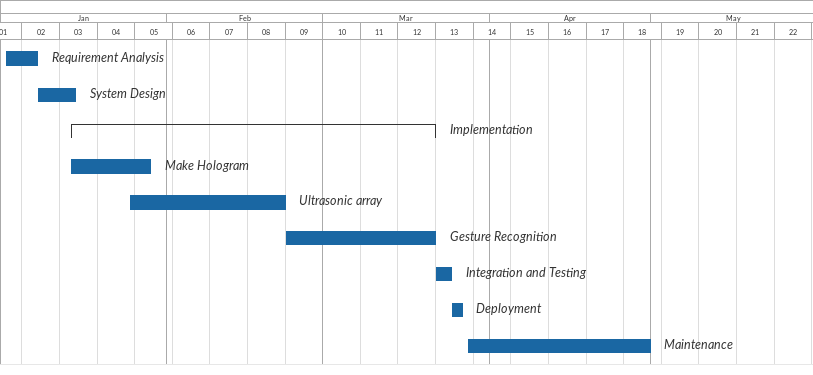
\includegraphics[scale=.5]{images/work_plan.png}
        \caption{Work Plan}
        \end{figure}
 \section{Budget}
    \renewcommand{\arraystretch}{1.3}
    \begin{center}
        \begin{table}[h]
            \begin{tabular}{ |c|c|c|c| }
                \hline
                Item & Price & Quantity & Total \\
                \hline
                Ultrasonic sensor & 350  & 100 & 3500 \\
                LCD display & 20000 & 1 & 20000 \\
                Transparent sheet & 200 & 4 & 800 \\
                Frame & 5000 & 1 & 5000 \\
                Micro-controllers + electronics & 1000 & 1 & 1000 \\
                LiDar + camera & 3000 & 1 & 3000 \\
                \hline
                \hline
                \textbf{Total:} &  & & 33,300\\
                \hline
                \end{tabular}
                \caption{Budget}
        \end{table}   
    \end{center}
    \chapter{Conclusion}

\par The device discussed here is system with a hologram display which can provide haptic feedback.The system will consist of an ultrasonic array to provide the feedback. While the use of camera and Machine Learning to track and read hand gestures.
\par After the literature survey, it has been determined that a phased array with about 64 transducers are sufficient for haptic feedback.
\par To implement the hologram display, Holographic plates which transmits 90\% of the light is used.He-Ne laser is used for this purpose.


\chapter{Reference}
[1]	Y. Zhao, S. Follmer, "A functional optimization based approach for continuous 3D retargeted touch of arbitrary complex boundaries in haptic virtual reality", Proc. CHI, pp. 544: 1-544: 12, 2018.
\newline
\newline
[2] Gotsch, D., Zhang, X., Merritt, T., and Vertegaal, R. Telehuman2: A cylindrical light eld teleconferencing system for life-size 3d human telepresence. In Proceedings of the 2018 CHI Conference on Human Factors in Computing Systems, ACM (2018), 522.
\newline
\newline
[3] Nakamura, T., Yano, T., Watanabe, K., Ishii, Y., Ono, H., Tambata, I., Furue, N. and Nakahata, Y., 2019, July. 360-degree transparent holographic screen display. In ACM SIGGRAPH 2019 Emerging Technologies (p. 1). ACM.
\newline
\newline
[4] Arroyo-Palacios, Jorge, Mahdi Azmandian, and Steven Osman. "Bringing Video Game Characters into the Real World on a Holographic Light Field Display." Proceedings of the 19th ACM International Conference on Intelligent Virtual Agents. ACM, 2019.
\newline
\newline
[5] Kim, Jin Ryong, et al. "Demonstration of Refinity: An Interactive Holographic Signage for New Retail Shopping Experience." Extended Abstracts of the 2019 CHI Conference on Human Factors in Computing Systems. ACM, 2019
\newline
\newline
[6] A. Marzo, T. Corkett, and B. W. Drinkwater, “Ultraino: An open phased-array system for narrowband airborne ultrasound transmission,” IEEE Trans. Ultrason., Ferroelectr., Freq. Control 65(1), 102–111 (2017)
\end{document}
